% Name: Stem plot
% Description: A discrete-time signal x[n], a sampled decaying cosine, drawn as stems from the axis with a dot at each sample.
% Tags: stem plot, discrete signal, sampling, signal processing

\usepackage{pgfplots}
\pgfplotsset{compat=1.18}

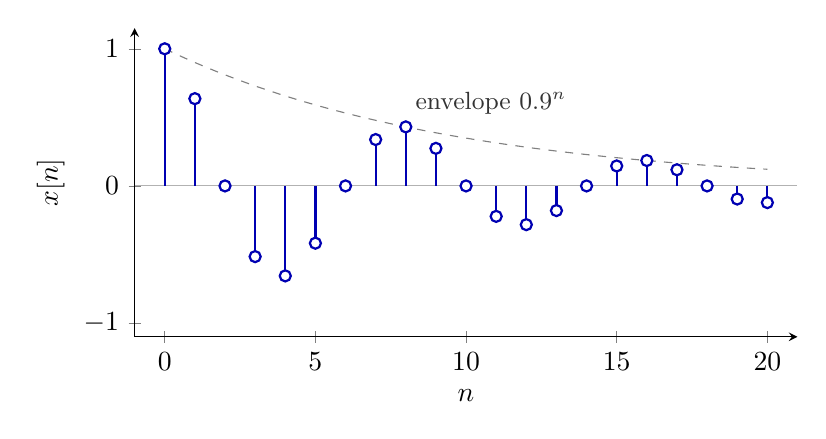
\begin{tikzpicture}
  \begin{axis}[
    width=10cm, height=5.5cm, axis lines=left,
    xlabel=$n$, ylabel={$x[n]$}, xmin=-1, xmax=21, ymin=-1.1, ymax=1.15,
    xtick={0,5,...,20}, ytick={-1,0,1},
  ]
    \draw[gray!60] (axis cs:-1,0) -- (axis cs:21,0);
    \addplot[ycomb, blue!70!black, thick, mark=*, mark options={fill=white}, domain=0:20, samples=21]
      {0.9^x*cos(deg(pi*x/4))};
    \addplot[gray, dashed, domain=0:20, samples=60] {0.9^x};
    \node[gray!40!black, font=\small, anchor=south west] at (axis cs:8,0.45) {envelope $0.9^n$};
  \end{axis}
\end{tikzpicture}
